%\documentclass[tikz, border=5pt]{standalone}
\begin{document}
	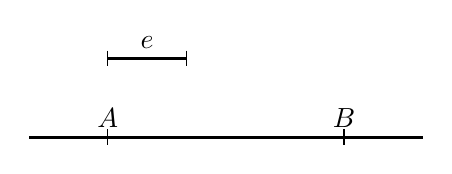
\begin{tikzpicture}
		% 绘制水平直线
		\draw[line width=1pt] (-2,0) -- (3,0);
		
		% 点A:标记文字、小竖线
		\node at (-1,0) [above] {$A$};
		\draw (-1,0.1) -- (-1,-0.1);  % A点的垂直小竖线(上下各延伸0.1单位)
		
		% 点B:标记文字、小竖线
		\node at (2,0) [above] {$B$};
		\draw (2,0.1) -- (2,-0.1);  % B点的垂直小竖线
		
		% 上方线段e:线段本身、两端小竖线、标记文字
		\draw[line width=1pt] (-1,1) -- (0,1);
		\draw (-1,1.1) -- (-1,0.9);  % e线段左端的垂直小竖线
		\draw (0,1.1) -- (0,0.9);  % e线段右端的垂直小竖线
		\node at (-0.5,1) [above] {$e$};
	\end{tikzpicture}
\end{document}
